% !TEX root = ../main.tex

\chapter{Publications}
\label{app:pub}

This chapter includes copies of the following publications and talks:

\todo{finish list here}

Funding was provided to attend ISCC 2016 in Oxford by Jon Bennett, Clinton Ingrams and a Graduate School Travel Award.

A travel fund has been awarded by the DMU Faculty of Technology for travel to Australia, Sydney for the Creativity and Cognition conference in July 2013.

De Montfort University has granted me a full 3 year bursary covering living costs and tuition fees.

\spirals

\todo{update}

IOCT Student Showcase 07 June 2016

Conference talk on ``Creative Zombie Apocalypse'' (by Fania Raczinski and Dave Everitt) at ISCC in Oxford, UK, 29 March 2016.

Phoenix CAS talk on ``Pata-computed Poetry'' in Leicester, UK, 14 Oct 2015.

De Montfort University Leicester Media School Launch Showcase, 05 November 2014.

De Montfort University Institute of Creative Technologies PhD showcase at the Phoenix Cube Gallery, Leicester, 15--18 August 2014.

Conference talk on ``'' at Creativity and Cognition in Syndey, Australia, 20 June 2013.

TDC talk on ``The Pataphysics of the Future'' (by Andrew Hugill, Hongji Yang and Fania Raczinski) in Leicester, UK, 13 Feb 2013.


\begin{enumerate}
  \item Talk given at IEEEISCC'16 in Oxford, UK (March/April 2016).
  \item Conference paper `Creative Zombie Apocalypse: A Critique of Computer Creativity Evaluation'. Proceedings of 2nd IEEE International Symposium of Creative Computing (2016).
  \item Presentation slides for a \gls{cas} \gls{ioct} talk at the Phoenix in Leicester, UK (14 Oct 2015).\footnote{\url{http://interactlabs.co.uk/news/2015/10/ioct-talks---videos-now-available}, \url{https://vimeo.com/142947457}}
  \item \gls{ioct} \gls{lms} Showcase, \gls{dmu}, Leicester, UK (5 Nov 2014).
  \item \gls{ioct} PhD Research Showcase, Phoenix Cube, Leicester, UK (15-18 Aug 2014).\footnote{Sean's Gallery \url{https://www.flickr.com/photos/seancuttlefish/sets/72157646116801940/}, Interact Blog \url{http://interactlabs.co.uk/diary/2014/08/dmu-phd-showcase}}
  \item Journal article `The pataphysics of creativity: developing a tool for creative search'. Routledge: Digital Creativity, Volume 24, Issue 3 (2013).
  \item Talk given at Creativity and Cognition conference in Sydney, Asutralia (20 June 2013).\footnote{\url{http://cc13.creativityandcognition.com/}}
  \item Conference paper `Creative Search Using Pataphysics'. Proceedings of the 9th ACM conference on Creativity and Cognition (2013).
  \item \gls{tdc} \gls{dmu} Talk, Leicester, UK (13 Feb 2013).\footnote{\url{https://www.youtube.com/watch?v=UxYUZMyPE0o}}
  \item Conference paper `A Framework for Creativity in Search Results'. Proceedings of the 3rd International Conference on Creative Content Technologies (2011).
'.
\end{enumerate}

\phantomsection
\addtocounter{section}{1}
\addcontentsline{toc}{section}{\protect\numberline{\thesection}IEEE ISCC 16 Conference paper}
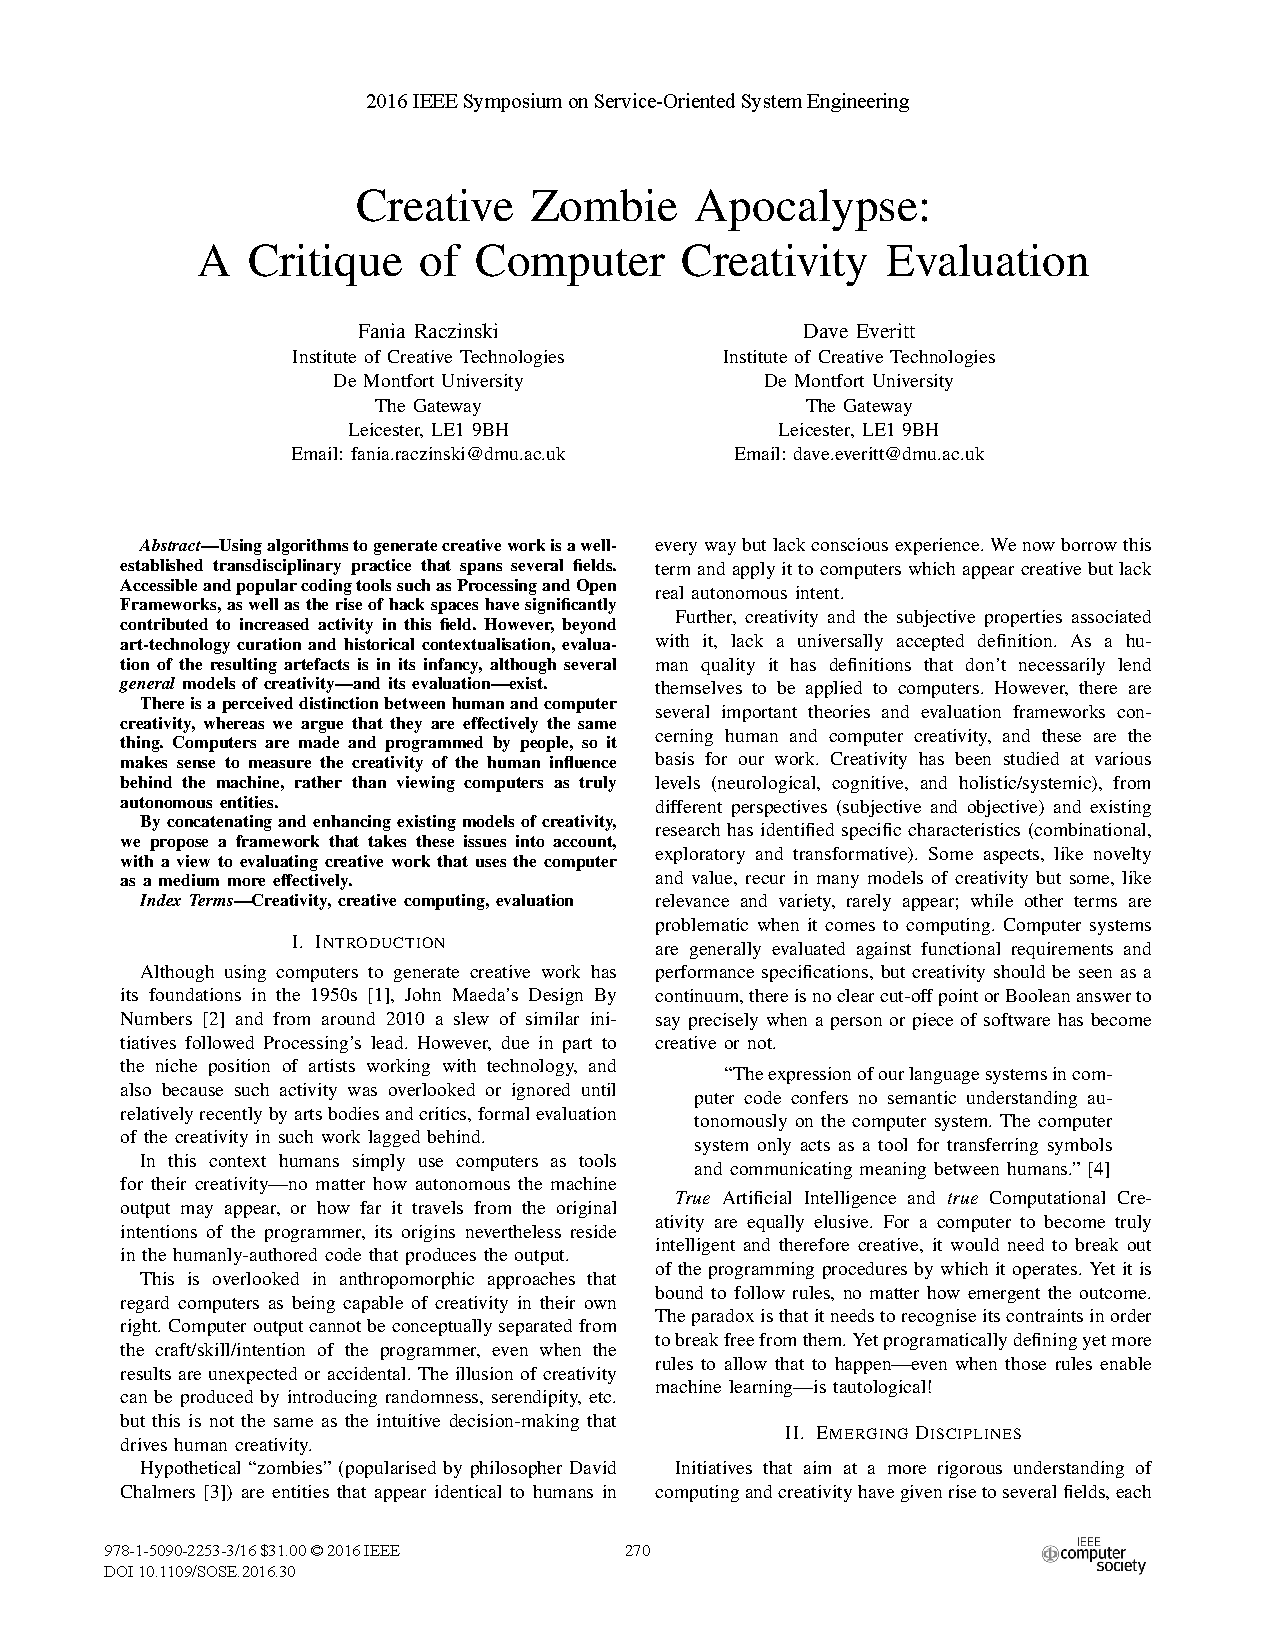
\includepdf[pages=-, nup=2x3, frame, scale=.8, pagecommand={\thispagestyle{plain}}]{RaczinskiEveritt.pdf}


\phantomsection
\addtocounter{section}{1}
\addcontentsline{toc}{section}{\protect\numberline{\thesection}IOCT CAS talk at Phoenix}
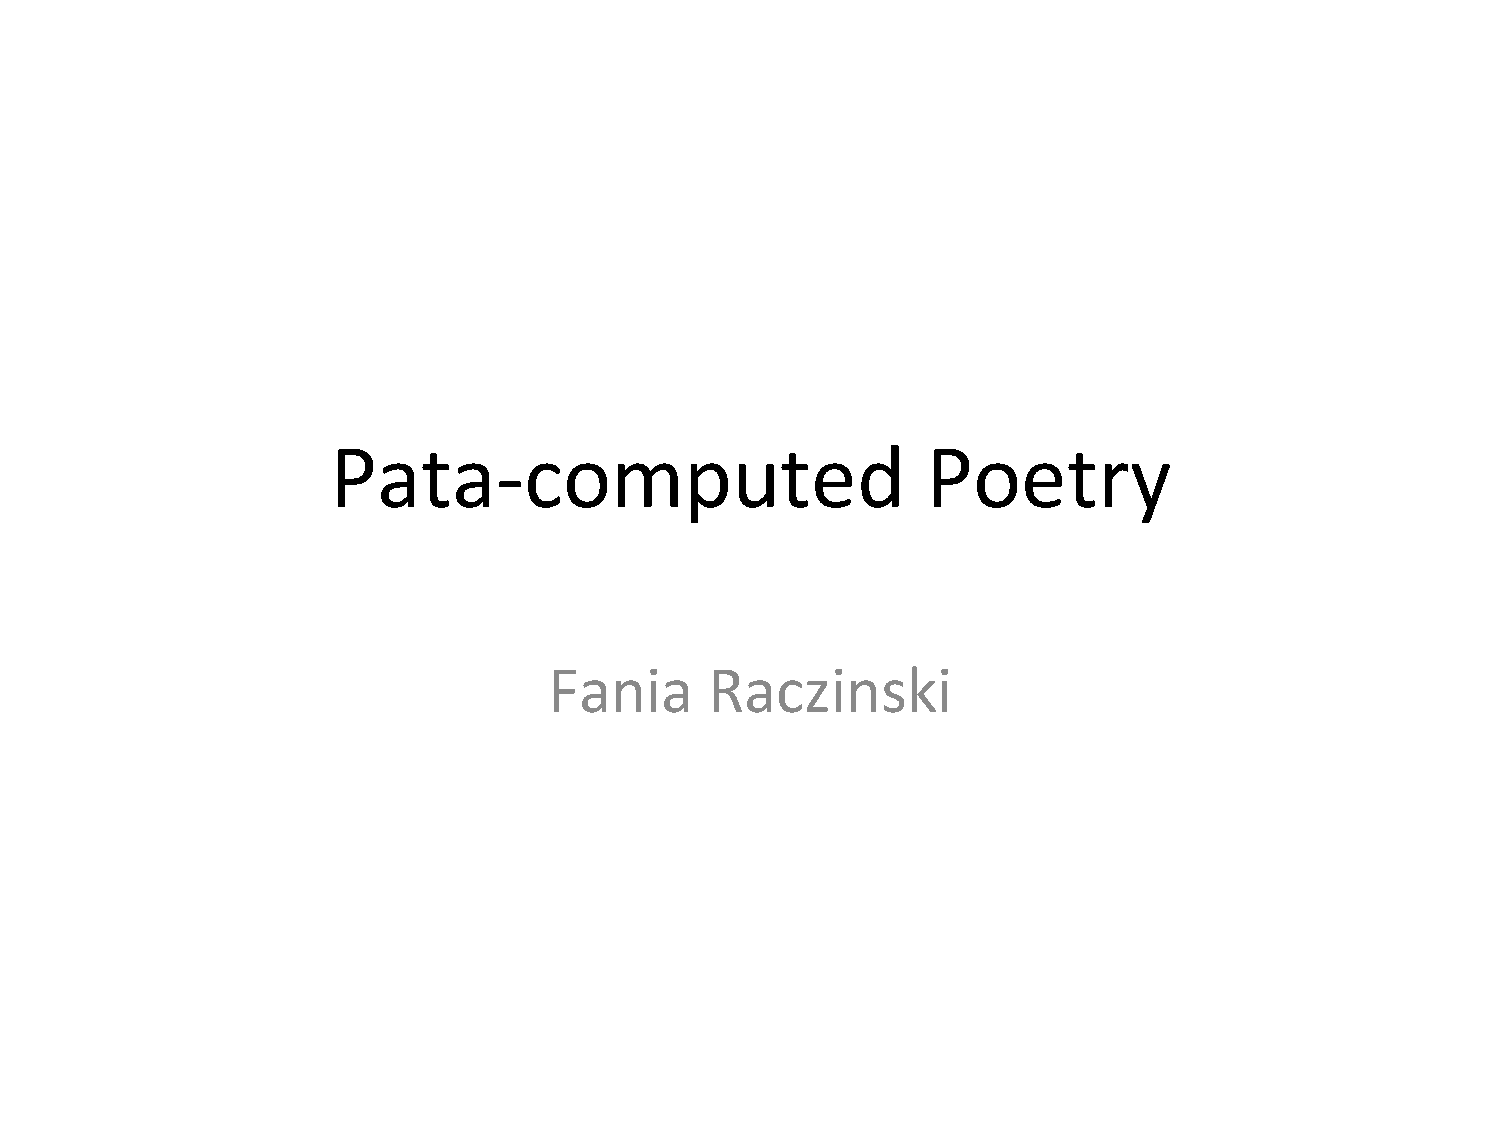
\includepdf[pages=-, nup=2x3, frame, scale=.8, pagecommand={\thispagestyle{plain}}]{CASTalk2015.pdf}


\phantomsection
\addtocounter{section}{1}
\addcontentsline{toc}{section}{\protect\numberline{\thesection}IOCT LMS Showcase}
- IOCT LMS Showcase. 5 Nov 2014.
<!-- ![Tweets](Citations/tweets.png) -->
\newpage


\phantomsection
\addtocounter{section}{1}
\addcontentsline{toc}{section}{\protect\numberline{\thesection}IOCT PhD Showcase at Phoenix}
Phoenix Exhibit.
Phoenix Cube Showcase. 15-18 Aug 2014. [Sean's Gallery](https://www.flickr.com/photos/seancuttlefish/sets/72157646116801940/), [Interact Blog](http://interactlabs.co.uk/diary/2014/08/dmu-phd-showcase)
\newpage


\phantomsection
\addtocounter{section}{1}
\addcontentsline{toc}{section}{\protect\numberline{\thesection}The pataphysics of creativity journal article}
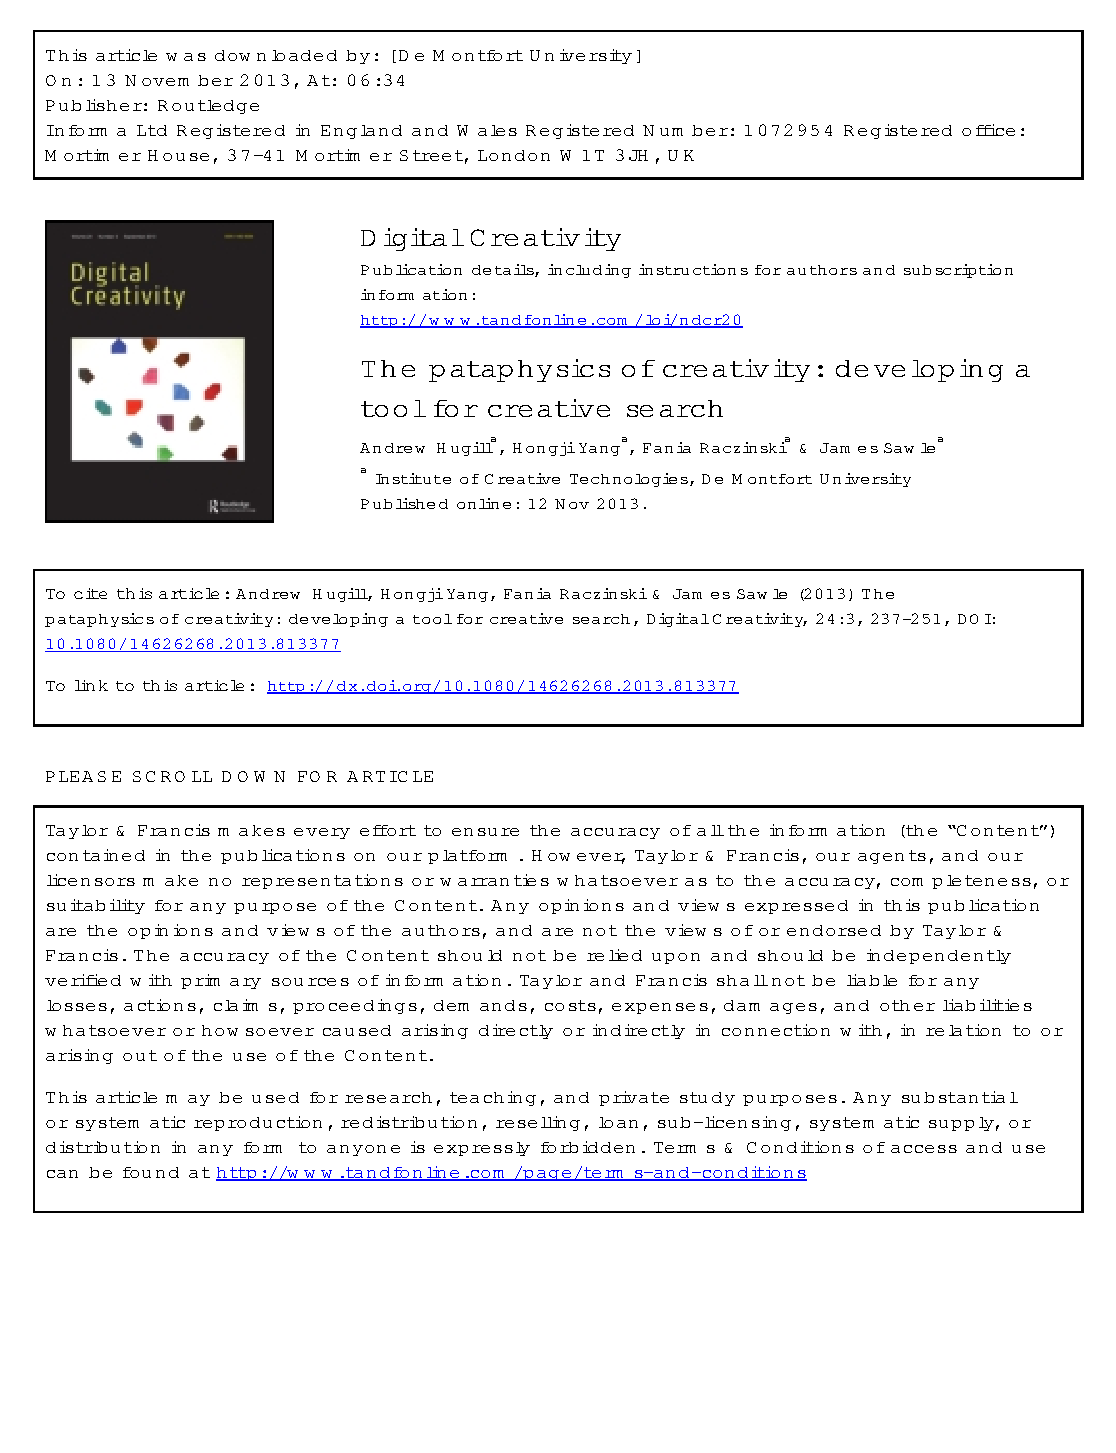
\includepdf[pages=-, frame,scale=.8, pagecommand={\thispagestyle{plain}}]{HugillYangRaczinskiSawle.pdf}


\phantomsection
\addtocounter{section}{1}
\addcontentsline{toc}{section}{\protect\numberline{\thesection}Creativity and Cognition conference talk}

\includepdf[pages=-, nup=1x3, frame,scale=.8, pagecommand={\thispagestyle{plain}}]{CC13Talk2013.pdf}


\phantomsection
\addtocounter{section}{1}
\addcontentsline{toc}{section}{\protect\numberline{\thesection}Creative Search Using Pataphysics conference paper}
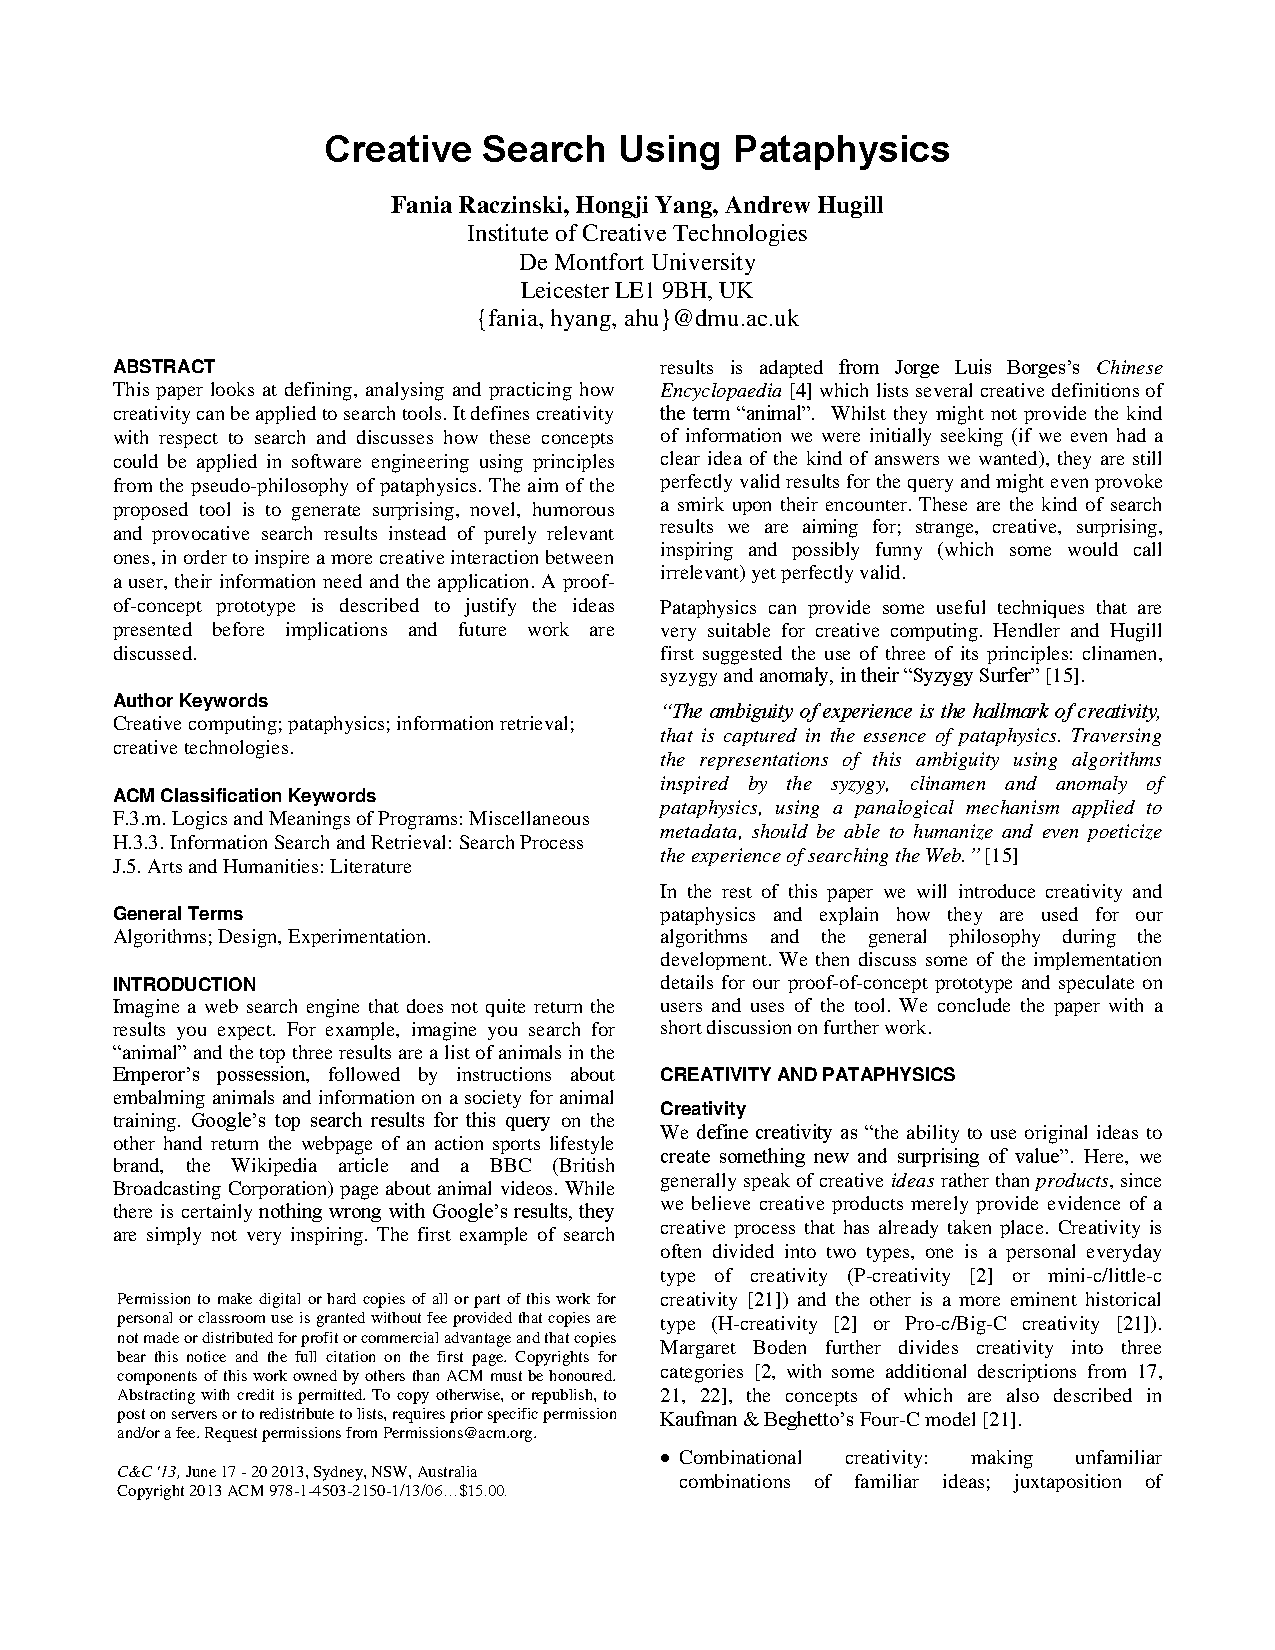
\includepdf[pages=-, frame,scale=.8, pagecommand={\thispagestyle{plain}}]{RaczinskiYangHugill.pdf}


\phantomsection
\addtocounter{section}{1}
\addcontentsline{toc}{section}{\protect\numberline{\thesection}IOCT TDC talk}
TDC Talk Andrew Hugill
\newpage


\phantomsection
\addtocounter{section}{1}
\addcontentsline{toc}{section}{\protect\numberline{\thesection}A Framework for Creativity in Search Results conference paper}
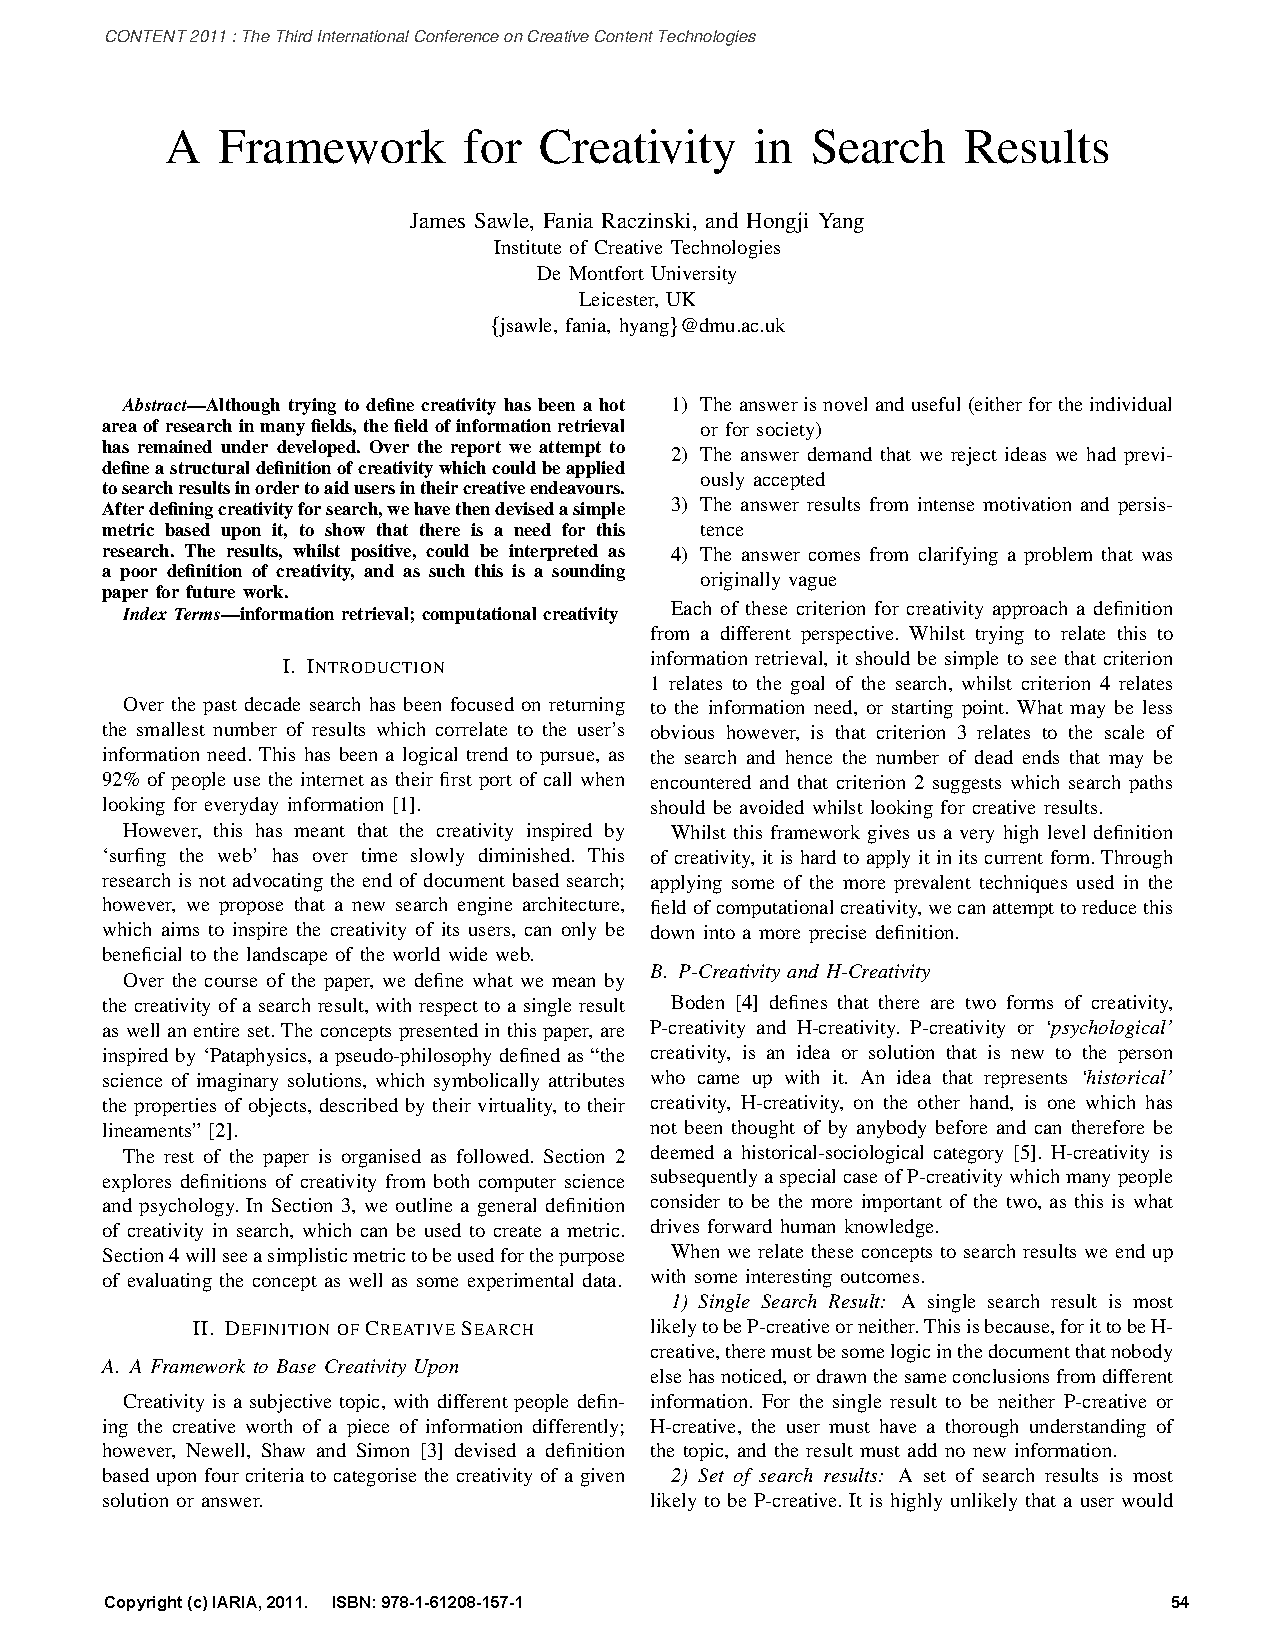
\includepdf[pages=-, frame,scale=.8, pagecommand={\thispagestyle{plain}}]{SawleRaczinskiYang.pdf}
